\chapter{A kiberbiztonsági analízis metodológiája}

A diplomamunkám legfontosabb része a metodológia előállítása volt. A metodológia az ami biztosítja azoknak a céloknak az elérését, hogy az analízis (i) teljes körű legyen, (ii) megismételhető legyen és (iii) már létező információkra építsen, azon túl, hogy az eredménye és használata minél átláthatóbb legyen a stakeholderek és az elemző mérnök számára is.

Ez a metodológia kapcsolja össze az autóiparra jellemző rendszermodelleket a fenyegetésmodellekkel. Ennek segítségére és támogatására készült el a kapcsolódó modellező eszköz és ennek az eredménye az egyik legfontosabb előállított értéke a kiberbiztonsági mérnök feladatkörnek.

Az említett fejezetben a példáimat egy tetszőleges személygépjármű kormányrendszerének az aktuációs (actuation: mozgásba hoz működtet) funkcionalitására készítettem el. 

Az \textit{Áttekintés} fejezet tartalmaz egy magas szintű végigvezetést a bemenetektől a kimenetig és a közte megtett lépésekről.

A \textit{Termékleírás és fenyegetésmodell származtatása} mutatja be a kiindulómodell elkészítésének lépéseit valamint, hogy abból, hogyan állítjuk elő a fenyegetés modellt.

A \textit{Fenyegetésmodellezés} fejezetben láthatóak a további lépések a fenyegetésmodell specifikálására, valamint be mutatja a fenyegetésmodellből előállított támadási fák konstrukcióját és annak szerkesztésének lépéseit.

A \textit{Dokumentumok generálása és manuális analízis} fejezetben pedig találhatóak a szabvány által előírt output előállítása és az elemző eszköz használatát követő folyamatok.

\section{Áttekintés}

A metodológiám fő feladata a \textit{Háttérismeretek} fejezetben található \textit{Követelmények a fenyegetéselemzésre és kockázatértékelésre} részben leírtakat követve kialakítsam azt a lépéssorozatot amelyet az általam fejlesztett eszköz támogatásával végre lehet hajtani és el lehet jutni egy általános autóipari modellből a kockázatelemzés eredményéig.

A lépésekről egy áttekintés a \ref{fig:04_OVERVIEW} ábrán látható. Itt egyrészről a fehér hátterű négyzetekben az ISO 21434 által definiált lépések láthatóak amelyek bővebb leírása a \textit{Háttérismeretek} részben található, lila hátterű négyzetekben pedig az ebben a fejezetben bemutatott lépések láthatóak. Így látható egy egyszerűbb áttekintés a két módszertan közti fedettségről.

\begin{figure}[!ht]
	\centering
	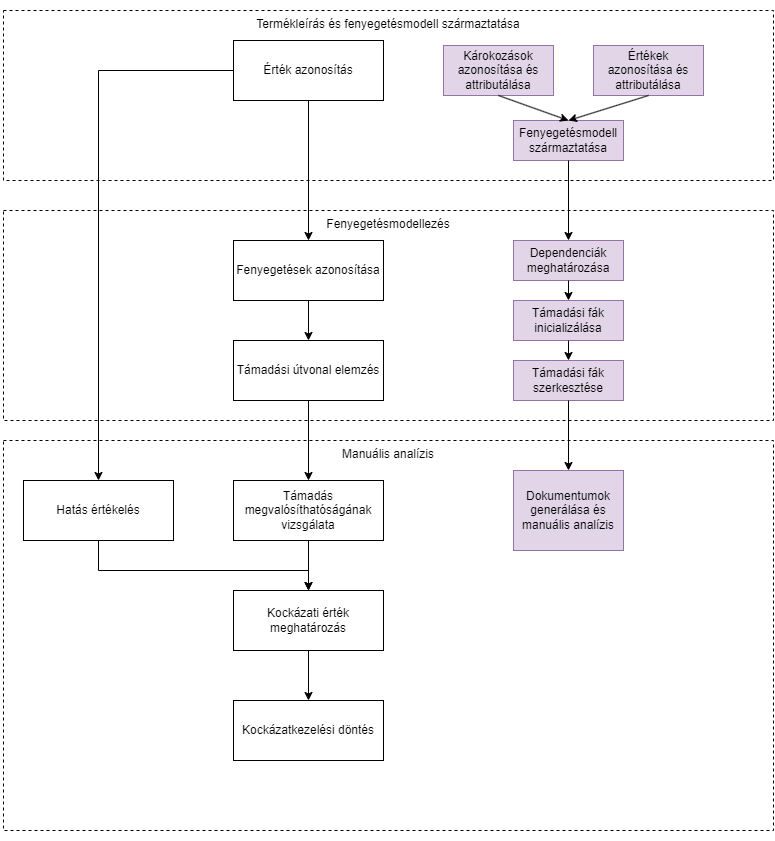
\includegraphics[width=130mm, keepaspectratio]{figures/04_overview.png}
	\caption{Metodológia áttekintése}
	\label{fig:04_OVERVIEW}
\end{figure}

\section{Termékleírás és fenyegetésmodell származtatása}

Ez a fejezet mutatja be az első lépéseit a kockázatelemzési folyamatnak. Itt lesz szükségünk a kiinduláskor rendelkezésünkre álló termékleírást (ami a rendszermodell egy részhalmaza) bővíteni kiberbiztonsági attribútumokkal majd abból származtatni egy olyan új modellt ami a kiberbiztonsági elemzésre alkalmas lesz.

Ehhez a rendszermodellünkben két diagram típusra lesz szükség. Az egyik a viselkedési diagramok közé sorolható használati eset (use case) diagram, a másik pedig egy strukturális kategóriába sorolható komponens diagram.\\

\subsection{Károkozások azonosítása és attributálása}

A használati eset diagramot a továbbiakban nevezzük \textit{kihasználási eset (abuse case)} diagramnak. Ez annyiban módosítja az eredeti diagram használatát, hogy amíg a szintaktikailag és szemantikailag ugyanaz, tartalmilag nem a felhasználó és rendszer közti kapcsolatokat keressük, hanem a támadó lehetséges motivációját és amit ténylegesen meg is tud tenni a rendszerrel. 

A kihasználási esetek azonosításában már tudjuk használni a CIA triád alkalmazását is. A bemutatott eljárásban, veszünk egy funkcionalitást amit a vizsgált termék ellát és azt finomítjuk tovább az egyes kiberbiztonsági tulajdonságoknak a sérülése szerint. Egy példa a \ref{fig:04_abuse_case} ábrán látható.

\begin{figure}[!ht]
	\centering
	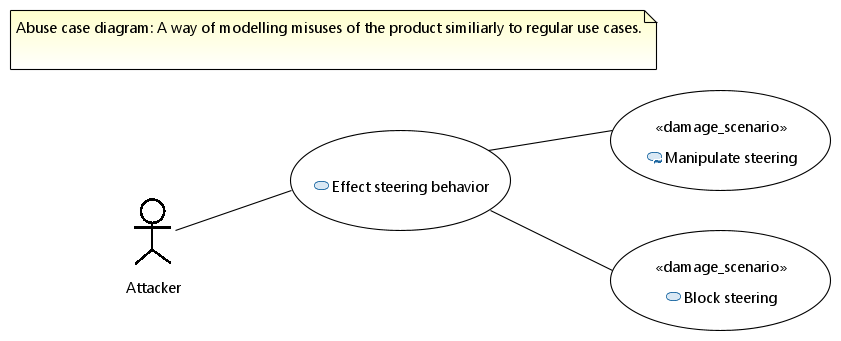
\includegraphics[width=130mm, keepaspectratio]{figures/04_abuse_case.png}
	\caption{Példa kihasználási eset diagramra}
	\label{fig:04_abuse_case}
\end{figure}

A példán jól látható, hogy amíg az "Effect steering behavior" tekinthető is lenne elvárt működésnek egy kormányrendszer esetén, addig amikor ez egy támadó lehetséges céljai közé tartozik akkor már nevezhető ez egy kihasználási esetnek. Ezt tudjuk tovább finomítani aszerint, hogy mely kiberbiztonsági tulajdonság sérülhet. Az eljárásban használt tulajdonságok a bizalmasság, sértetlenség és elérhetőség, ezek bővebben a \textit{Háttérismeretek} fejezetben kerültek bemutatásra. A "Manipulate steering" esetében az aktuáció sértetlenségi attribútuma sérül, a "Block steering" esetén pedig az elérhetősége. Bizalmassági tulajdonsága nincsen az aktuációnak, hiszen ennek a működtetése kívülről nem igényel semmilyen személyes adatot, szellemi terméket vagy kriptográfiai információt.

Az ISO 21434 szerint mivel ez a kihasználási eset (i) összeköt egy funkcionalitást egy nem kívánt következménnyel, valamint ezáltal (ii) értékekhez lesz köthető, emiatt jelölhetjük ezt egy \textit{károkozásnak} (damage scenario). \\

\subsection{Értékek azonosítása és attributálása}

A komponens diagram lesz, az ISO 21434 megnevezése szerint, a termékleírás (item definition). Ennek célja, hogy meghatározzuk a (i) termék határait, (ii) a termék funkcionalitását, illetve a (iii) kezdeti architektúrát.

A termék határai, vagy kiberbiztonsági fogalommal támadási felületet (attack surface), a felvett HW komponensek formájában vagy a beérkező üzenetek (információk) formájában értékként vehetjük fel, a funkcionalitással egyetemben. Az előbbi kettő szintén analizálhatóak a kiberbiztonsági tulajdonságaik alapján (pl: bizalmas információt szállít-e egy CAN üzenet), a funkcionalitásnál erre nincsen szükség hiszen a károkozásokból származtatható lesz egy funkcionalitás védendő tulajdonsága.

A kezdeti architektúra abban az értelemben van figyelembe véve, hogy a termékleírás maga egy komplexebb rendszermodell esetre is alkalmazható, ahol a rendszermodell egyes komponenseit jelöljük fel az előbbi három sztereotípia egyikével.

Erre példa a \ref{fig:04_item_definition} ábrán látható.

\begin{figure}[!ht]
	\centering
	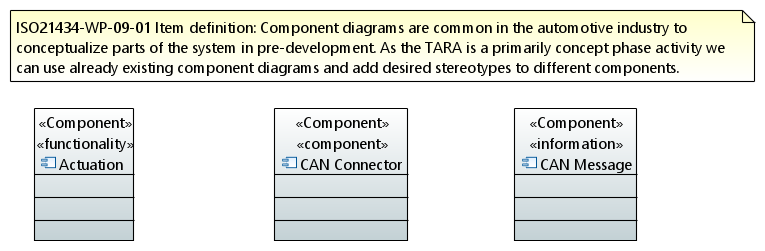
\includegraphics[width=130mm, keepaspectratio]{figures/04_item_definition.PNG}
	\caption{Példa termékleírásra}
	\label{fig:04_item_definition}
\end{figure}

A termékleírásban látható, hogy az Actuation mint funkcionalitás jelenik meg, a CAN csatlakozó mint HW komponens, a buszon szállított és a csatlakozón beérkező CAN üzenetek pedig mint információ. 

\subsection{Fenyegetésmodell származtatása}

Ebből a két diagram típusból, ami bármely autóipari termék rendszermodelljéhez könnyen integrálható, most már tudunk származtatni olyan modellt amely a fenyegetésmodellezési eljárásunkhoz szükséges. Ehhez nincsen másra szükségünk mint, hogy készítsünk egy kivonatot az elébb feljelölt információkból, amelyet aztán a fenyegetésmodellező eszközünk fel tud használni bemenetként.

Valamint fontos kiemelni az előző pontokban leírtak végrehajtásával egyben végrehajtottuk az ISO 21434 által leírt \textit{Érték azonosítás} lépését is a kockázatelemzésnek.

\section{Fenyegetésmodellezés}

Már az előző fejezetben leírtak is fenyegetésmodellezésnek nevezhető, az még elsősorban a fenyegetésmodell előkészítését és a rendszermodellből való származtatását végezte el.

A következő fejezetben leírtak mutatják be magát a kiberbiztonsági analízisnek a menetét, aminek az eredménye a manuális analízisre alkalmas információk előállítása.

\subsection{Dependenciák meghatározása}

Első lépésként meg kell határoznunk a dependenciákat a károkozások, funkcionalitás és értékek között. Ezt egyszerűen megtehetjük, először a károkozásokat rendeljük hozzá egy-egy funkcionalitáshoz, majd pedig a funkcionalitásokhoz hozzárendeljük, hogy mely szoftveres információktól és mely hardver komponensektől függ.

Ennek a modellje a \ref{fig:04_dependencies} ábrán látható.

\begin{figure}[!ht]
	\centering
	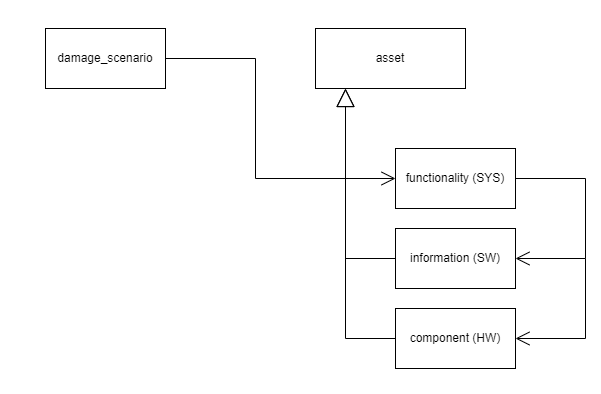
\includegraphics[width=130mm, keepaspectratio]{figures/04_dependencies.png}
	\caption{Károkozások, funkcionalitás és értékek összerendelése}
	\label{fig:04_dependencies}
\end{figure}

A korábbi példa esetében a két károkozásunk ("Manipulate steering", illetve "Block steering") az Actuation funkcionalitásnak a kártékony használatáról szólnak, ezzel már felvehető kapcsolat van a Károkozás és Funkcionalitás közt. 

Ezután határozhatjuk meg a további dependenciákat, a funkcionalitás eléréséhez szükséges egyrészről egy CAN csatlakozóhoz való hozzáférés (ez történhet a CAN buszon keresztül más ECU-n keresztül, vagy állóhelyzetben, olyan kialakítás mellett akár egy saját eszköz csatlakoztatásával). 

Másrészről pedig az aktuáció az alapján fog történni, hogy a kormányrendszer milyen üzeneteket kap a CAN buszról. Ilyen befolyásoló tényező lehet a jármű sebessége például.

\subsection{Támadási fák inicializálása}

A definiált következő lépése a szabványos kockázatelemzésnek a \textit{Fenyegetések azonosítása} és a \textit{Támadási útvonal elemzés}. 

Az előbbi elvégzésére a STRIDE keretrendszert fogom alkalmazni, amely az egyes fenyegetés típusokat rendeli a kiberbiztonsági tulajdonságokhoz, a keretrendszer bemutatása a \textit{Háttérismeretek} fejezetben található.

Az utóbbinak pedig ezzel együtt el tudjuk végezni az előkészítését, ahol a generált fenyegetéseket a meghatározott dependenciák szerint rendezzük.

\subsection{Támadási fák szerkesztése}

A támadási fák olyan irányított aciklikus gráfok amelyekben minden páratlan szinten egy fenyegetés vagy pszeudo-fenyegetés található, minden páros szintjén pedig egy logikai kapu amely lehet \textit{ÉS} vagy \textit{VAGY} típusú. A gyökér fenyegetést nevezhetjük rendszerszintű fenyegetésnek, a levélben lévőeket pedig szoftver- vagy hardverszintű fenyegetésnek. Ezek közé pszeudo-fenyegetéseket helyezhetünk el, ezzel csoportosítva a szoftver- vagy hardverszintű fenyegetéseket. 

További korlátozás a gráffal szemben, hogy minden fenyegetésnek 0 vagy egy kapuja lehet mint gyermek elem, illetve egy kapunak 1 vagy több gyermek fenyegetése lehet. A fenyegetés felfele nulla vagy egy kapuhoz csatlakozhat (ez már következik a gráf aciklikusságából), a kapunak felfele pedig pontosan egy fenyegetése kell, hogy legyen. Ebből következik, hogy egy fenyegetés gyökérnek számít, ha nincs felette kapu, pszeudónak ha felette és alatta is van kapu, levélnek pedig, ha nincs alatta kapu.

Ezeknek a fáknak a konstrukcióját úgy végezzük el, hogy minden károkozáshoz egy támadási fát rendelünk, annak a gyökér eleme a hozzá rendelt funkcionalitás valamint a károkozásban sérült tulajdonság alapján meghatározott fenyegetés. A levél elemeket szintén a funkcionalitáshoz rendelt értékekből és azok tulajdonságaiból kaphatjuk meg.

Ezután adhatunk hozzá a fához kapukat és határozhatjuk meg az összefüggéseket a szoftver- és hardverszintű fenyegetések valamint a rendszerszintű fenyegetés között.

Egy példa erre a fejlesztett elemző eszközben a \ref{fig:04_attack_tree} ábrán láthatunk.

\begin{figure}[!ht]
	\centering
	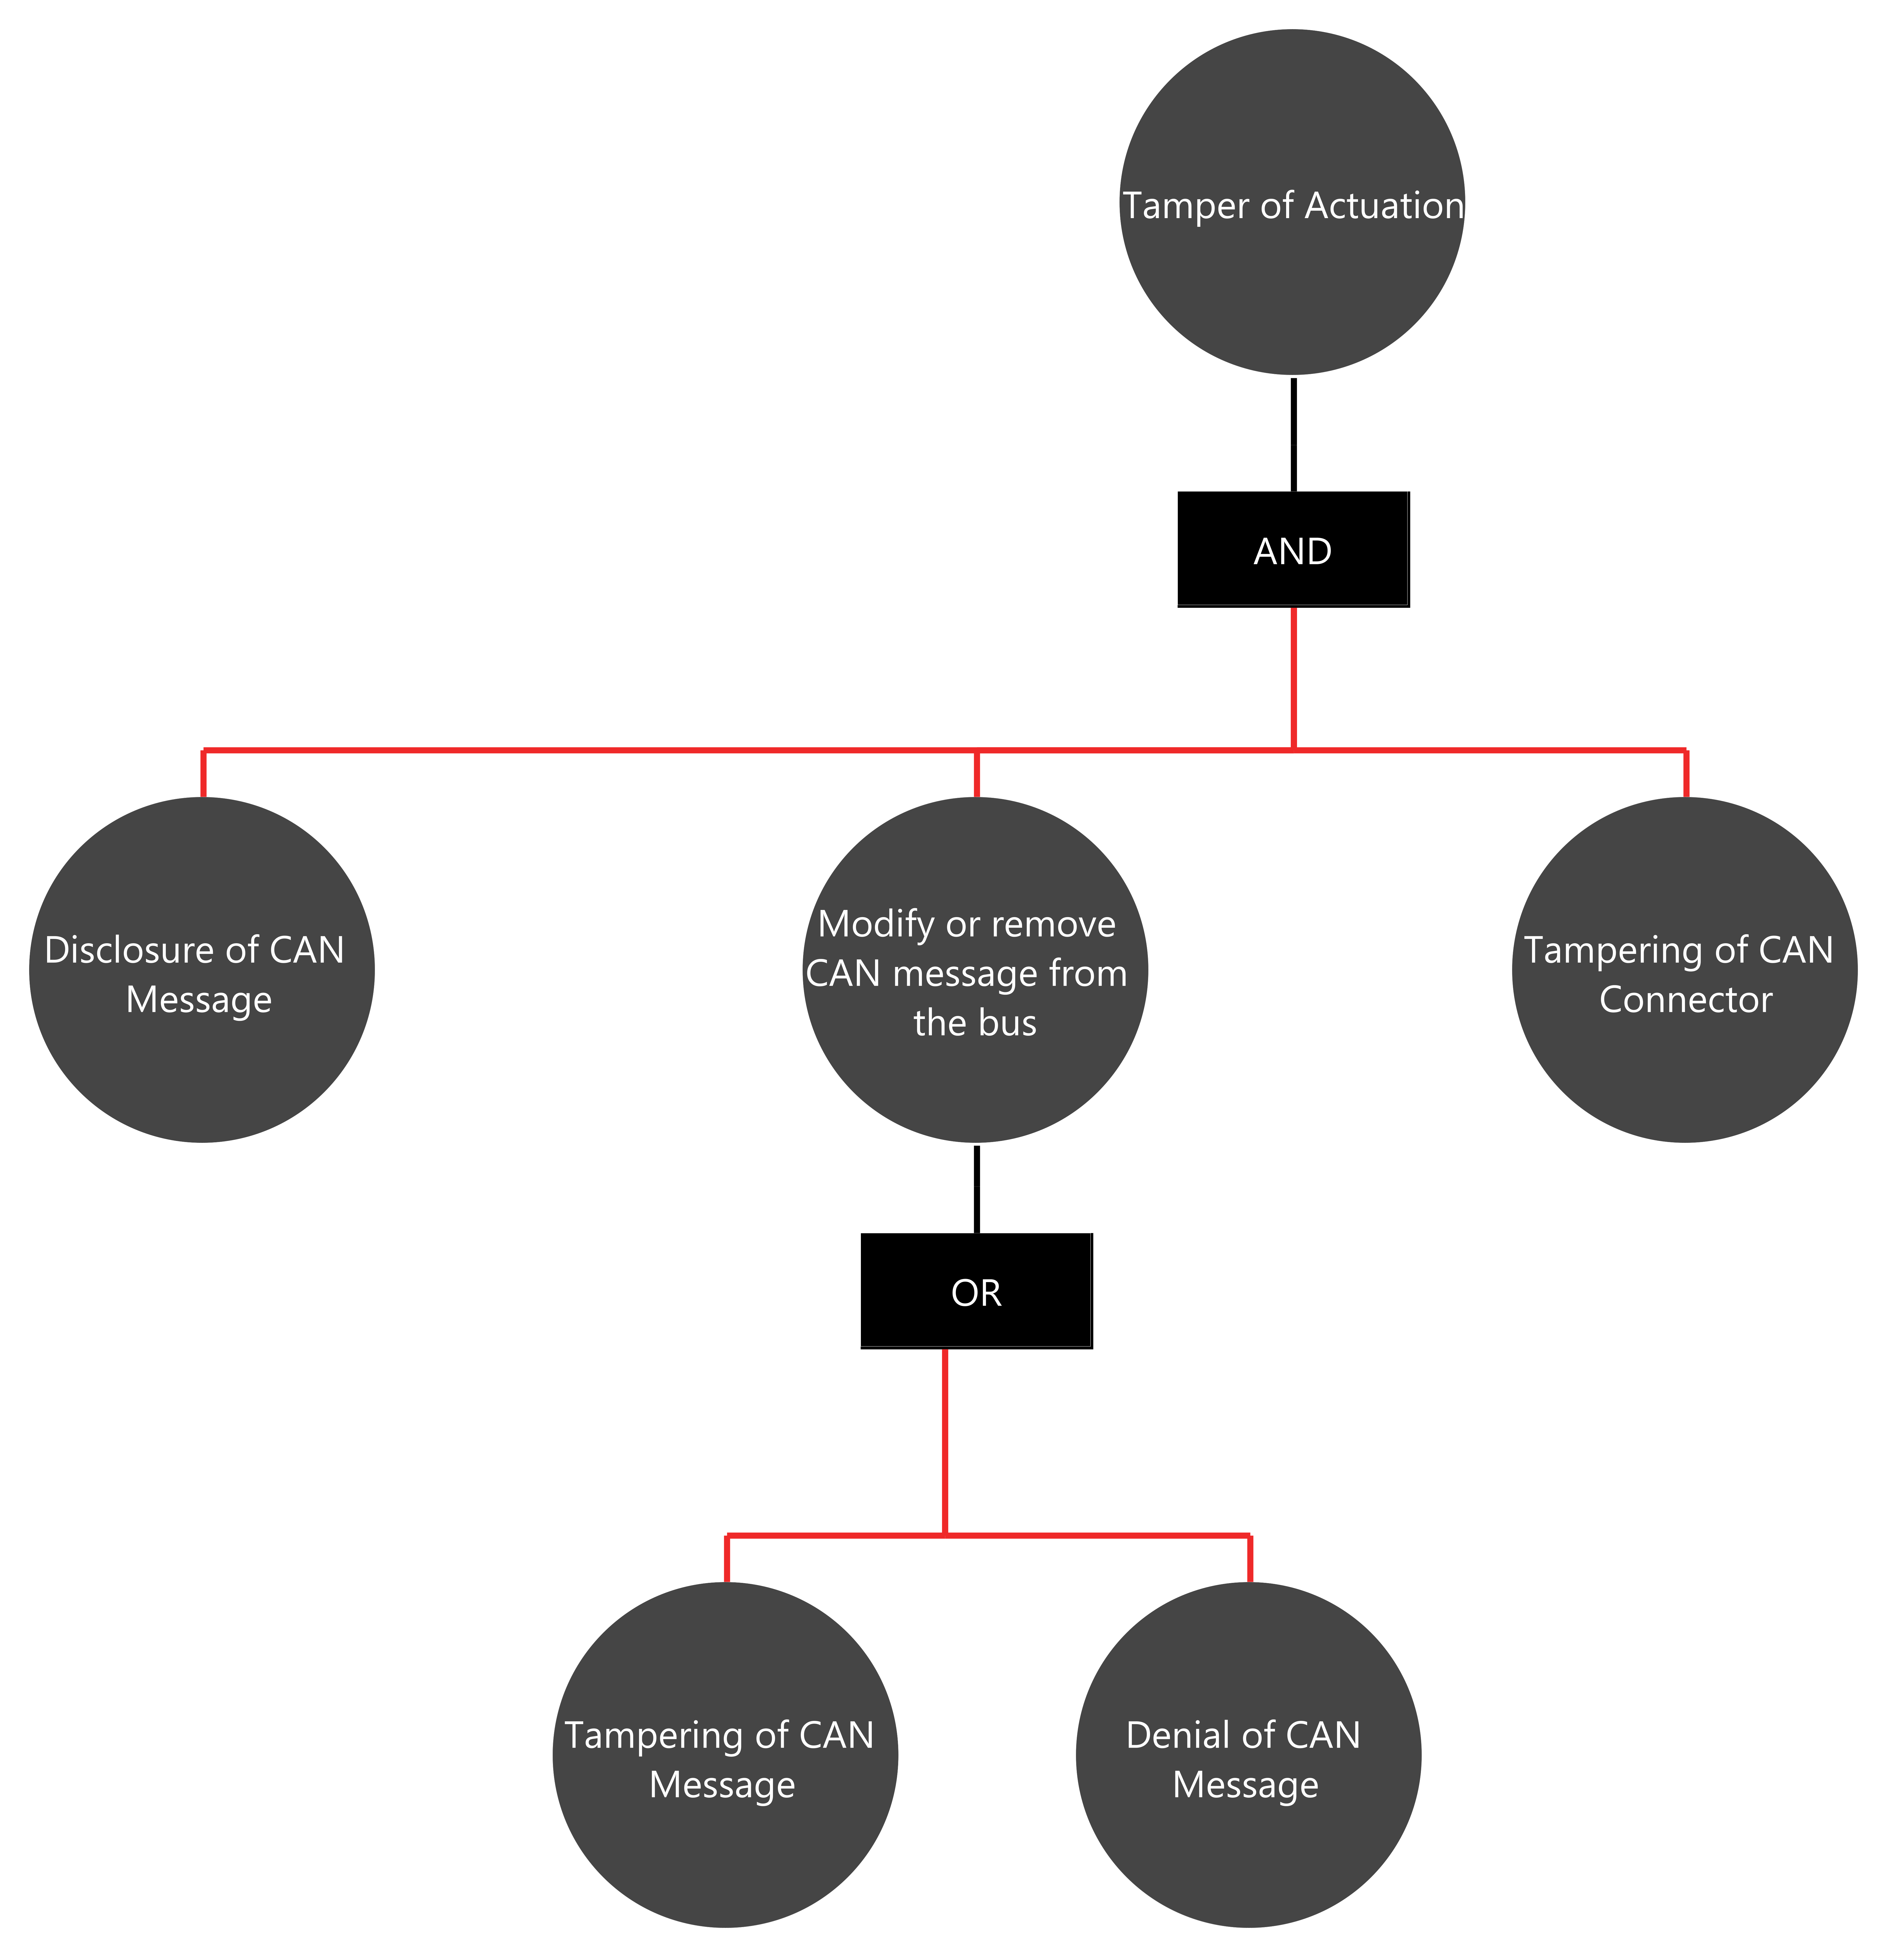
\includegraphics[width=130mm, keepaspectratio]{figures/04_attack_tree.png}
	\caption{Példa a támadási fára a "Manipulate steering" károkozáshoz}
	\label{fig:04_attack_tree}
\end{figure} 

Itt látható, hogy a támadási végrehajtásához szükséges egyrésről a CAN üzenet tartalmának megismerése, ez alapján tud a támadó saját üzeneteket konstruálni, megtalálni a címezhető ECU-kat, stb. 

Másrészről szükséges a CAN csatlakozó ellen a Tampering, ami a sértetlenség tulajdonság sértése. Erre példa, hogy amennyiben módosítani akarjuk a kerekek állását, azt befolyásolhatjuk a CAN csatlakozó abban az esetben, ha van hozzáférésünk a CAN buszhoz amire az ECU csatlakoztatva van.

Utolsó sorban pedig a CAN üzenetnek módosíthatjuk a tartalmát vagy annak a továbbítását tudjuk blokkolni bizonyos esetekben, ezek közül bármelyik fenyegetés jelenléte a rendszerünkben okozhatja a rendszerszintű fenyegetés jelenlétét is.

Ennek a támadási fa konstrukciónak az elvégzése minden károkozásra elegendő ahhoz, hogy teljesítsük a \textit{Támadási útvonal elemzés} lépését a szabványosított eljárásnak. 

\section{Dokumentumok generálása és manuális analízis}

Jelenleg a fenyegetésmodellünk tartalmaz információt a rendszerre releváns károkozásokról, funkcionalitásról, értékekről, fenyegetésekről valamint a fákból származtatható a támadási útvonalakról.

Ennek a modellnek a segítségével fogunk tudni minden analízist amely pusztán a jellegéből fakadóan manuális analízisre szükséges.

Az egyik ilyen a hatás értékelés, ez a károkozások listázásával előállítható. A másik a támadás megvalósíthatóságnak a vizsgálata, amelyben a támadási útvonalak és támadási lépéseket kell kiértékelnünk a megvalósíthatóságuk szerint.

A támadási útvonal egy minimális halmaza a levéleseményeknek amelyeknek a teljesülése (rendszerben egy időben való jelenléte) vezet a gyökér esemény, vagy rendszerszintű fenyegetés jelenlétéhez. A támadási lépések az egyes levél események lesznek.

Példa a hatásérték analízisre a \ref{tab:impact_rating} táblázatban látható, a támadási megvalósíthatóság elemzésre pedig a \ref{tab:attack_feas} táblázatban.

A táblázat oszlopai a határérték analízis esetén az SFOP keretrendszert használják, a támadási megvalósíthatóságnál pedig az Attack Potential Based megközelítést.

\begin{table}[h]
	\centering
	\begin{tabular}{|l|l|l|l|l|l|}
		\hline
		Damage Scenario & Safety & Financial & Operational & Privacy & Impact \\ \hline
		Manipulate steering & ~ & ~ & ~ & ~ & ~ \\ \hline
		Block steering & ~ & ~ & ~ & ~ & ~ \\ \hline
	\end{tabular}
	\caption{Generált hatásérték analízis dokumentum}
	\label{tab:impact_rating}
\end{table}

\begin{table}[h]
\centering
\begin{tabular}{|l|l|l|l|l|l|l|}
	\hline
	Attack Paths & ET & SE & KoI & WoO & Eq & Attack Feasibility \\ \hline
	Attack Path - Manipulate steering & ~ & ~ & ~ & ~ & ~ & ~ \\ \hline
	|-> Tampering of CAN Message & ~ & ~ & ~ & ~ & ~ & ~ \\ \hline
	|-> Tampering of CAN Connector & ~ & ~ & ~ & ~ & ~ & ~ \\ \hline
	|-> Disclosure of CAN Message & ~ & ~ & ~ & ~ & ~ & ~ \\ \hline
	Attack Path - Manipulate steering & ~ & ~ & ~ & ~ & ~ & ~ \\ \hline
	|-> Denial of CAN Message & ~ & ~ & ~ & ~ & ~ & ~ \\ \hline
	|-> Tampering of CAN Connector & ~ & ~ & ~ & ~ & ~ & ~ \\ \hline
	|-> Disclosure of CAN Message & ~ & ~ & ~ & ~ & ~ & ~ \\ \hline
\end{tabular}
\caption{Generált támadás megvalósíthatósági elemzés dokumentum}
\label{tab:attack_feas}
\end{table}

Ezek a táblázatok már alkalmasak a megfelelő szakértők bevonásával az elemzés elvégzésére. Ezen eredményéből már meghatározható a kockázati érték és a kockázatkezelési döntés a stakeholder-ek által.